\documentclass[12pt]{article}
\usepackage[czech]{babel}
\usepackage[utf8]{inputenc}
\usepackage[IL2]{fontenc}
\usepackage{wrapfig}
\usepackage{graphicx}
\usepackage{cprotect}
\usepackage{amsmath}


\begin{document}
%\setlength{\parindent}{0pt}
\begin{titlepage}

\includegraphics[scale=0.2, trim=5cm 0 0 30cm]{logo.jpg}
\begin{center}
\vspace{5cm}
{\Huge
\textbf{KIV/PRO}\\
\vspace{1cm}
}
{\Large
\textbf{ROZPOZNÁVÁNÍ POZNÁVACÍCH ZNAČEK S POUŽITÍM ZPĚTNÉ PROPAGACE, NEURÁLNÍCH SÍTÍ A GENETICKÝCH ALGORITMŮ}
}
\end{center}
\vspace{\fill}

\begin{minipage}[t]{5cm}
\flushleft
Martin Hamet\\
\end{minipage}
\hfill
\begin{minipage}[t]{7cm}
\flushright
\today
\end{minipage}
\end{titlepage}

\tableofcontents
\newpage
\section{Abstrakt}
Účelem této práce je zhodnocení efektivity a hledání optimálních parametrů neuronové sítě s využitím genetických algoritmů. Pro zpracování obrázků byly použity metody pro konverzi do šedotónu, top-hat a binární morfologické transformace, dále metoda prahování Otsu a binární projekce. 

Výsledky ukazují že neurální sít optimalizovaná genetickými algoritmy se zpětnou propagací vyžaduje průměrně 2230 cyklů pro natrénování na daných mezích. Tento způsob je tedy o 36,83\% rychlejší než generická síť bez použité optimalizace genetickým algoritmem.

\section{Úvod}
Automatický rozpoznávací systém je určen jako náhrada za personální vyhodnocování v místech, kde je třeba znalostí, rozhodování a zkušeností. V našem případě se jedná o systém optického rozpoznávání znaků, který bez pomoci člověka dokáže rozpoznat a interpretovat znaky získané z fotografií poznávacích značek automobilů. Pro realizaci takového systému se nabízejí metody porovnávající vzory (SVM), neuronové sítě a podobně.

K nejpopulárnějším patří zmíněné neuronové sítě, které se pokouší simulovat biologické vlastnosti neuronů mozku. Jednotlivé neurony jsou navzájem propojeny s různými váhami tyto synapse v jistém smyslu uchovávají informaci, která se dá upravit trénováním. Jedním ze způsobů trénování neuronové sítě je zpětná propagace, kde je síti představována trénovací množina a vypočtené chyby při rozpoznávání se zpětně přenášejí synapsemi a upravují jejich váhy tak, aby příště byla chyba menší. Opakováním tohoto procesu se síť postupně učí rozpoznávat.

\pagebreak
\subsection{Neuronováí síť}
Rychlost trénování sítě je ovlivněna rychlostí učení a jeho momentem. Tyto dva atributy jsou úzce vázány na konkrétní síť a její použití. Optimální parametry nelze určit obecně. Atributy určují jak moc je síť náchylná k uvíznutí v lokálním optimu (nedosažení globálního optima). Rychlost učení při zpětné propagaci silně ovlivňuje také počet skrytých (vnitřních) neuronů sítě. Větší počet těchto neuronů umožňuje síti naučit se více informací za cenu delšího trénování. Ovšem příliš velký počet neuronů může vést k tzv. přeučení. Síť by v takovém případě nedokázala dobře zobecňovat a rozpoznávala by dobře pouze trénovací množinu a nic jiného.

Aby jsme získali optimální síť potřebujeme najít způsob jak určit tyto parametry. Pro určení optimálních hodnot lze použít metodu pokus-omyl, kdy náhodně nastavujeme parametry sítě a zkoušíme jejich úspěšnost. Tato metoda je ale časově náročná a vyžaduje interakci člověka.  Pro tento účel využijeme genetického algoritmu, kde se využívá přirozeného výběru. Vytvořením vektorů s náhodnými parametry sítě, které budou mutovat a křížit se navzájem. V každé generaci proběhne křížení a odstraní se nejslabší prvky generace. Postupným vyřazováním slabých kombinací získáme set optimálních nastavení.

\section{Předzpracování snímku}
V tomto kroku potřebujeme získat informace o vlastní poznávací značce z daného snímku.

Postup předzpracování:
\begin{itemize}
\renewcommand\labelitemi{--}
\setlength\itemsep{1px}
\item Změna rozměrů snímku na unifikovanou výšku 768px se zachováním poměru stran.
\item Převod snímku do šedotónu s ohledem na vnímání člověka. Jas pixelu získáme jako:
\begin{equation}
{ I }_{ Y }=0.30{ f }_{ R }+{ 0.59 }f_{ G }+{ 0.11 }f_{ B }\nonumber
\end{equation}
kde $f$ jsou jednotlivé barevné složky.

\item Odstranění reflexí pomocí top-hat\cite{Digital_image_processing} transformace.
\item Prahováním metodou Otsu\cite{Otsu_tresholding} získáme kandidáty pixelů znaků na poznávací značce (binární obraz viz levá část obr. \ref{H_projection}).
\item Provedeme operaci zavírání (eroze + dilatace maskou $2 \times 2$) pro odstranění malých defektů ve znacích (osamocené pixely, "praskliny", jemné výčnělky, ...). Dále provedeme erozi (maskou $3 \times 3$) kvůli ztenčení znaků po operaci zavírání.
\item Vertikální projekcí určíme nejširší pás ve snímku viz obr.\ref{H_projection} jako oblast příslušící znakům a ořízneme ze snímku přebytečné části.

\begin{figure}[h]
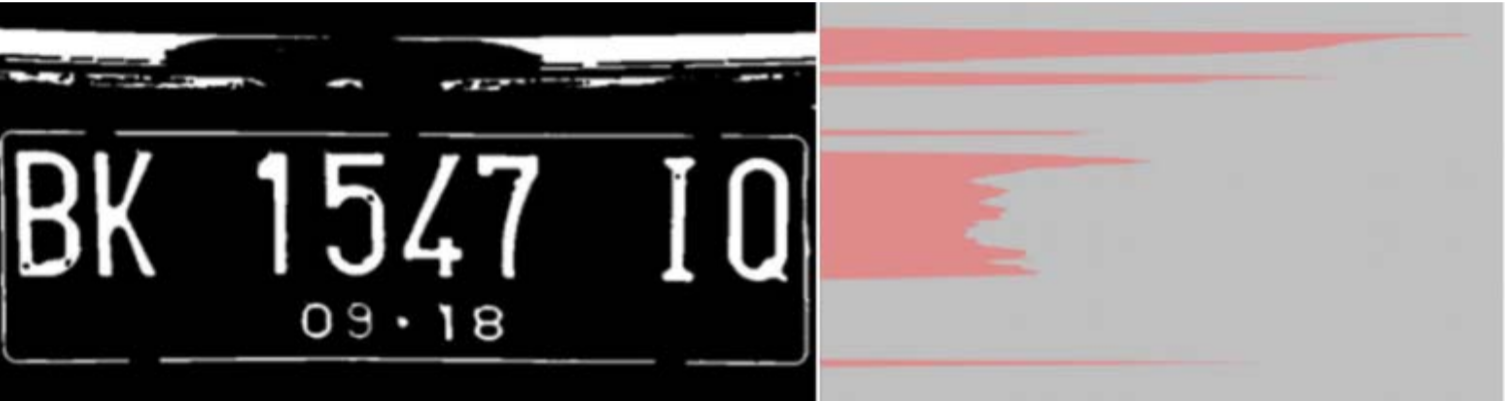
\includegraphics[width=15cm]{H_projection.png}
\caption{Vertikální projekce.}
\label{H_projection}
\end{figure}
\item Pro rozlišení jednotlivých znaků využijeme metody connected-component labeling z teorie grafů. Metoda nám poskytne všechny souvislé komponenty. Jednotlivé komponenty jsou dále separovány do segmentů ve snímku pomocí dat z jejich horizontálních projekcí (podobně jako u vertikální projekce). Správnost segmentace lze ověřit porovnáním poměrů výšky a šířky jednotlivých segmentů a jejich minimálních velikostí.
\item Kvůli zpracování jednotlivých znaků neuronovou sítí je nutné změnit rozlišení (rozměry) každého segmentu znaku, tak aby odpovídalo vstupu naší neuronové sítě. Rozměry $12\times9$ pixelů odpovídá 108 neuronům ve vstupní vrstvě sítě. Každý pixel náleží jednomu neuronu.
\item Aby hodnoty vstupu do sítě měli jednotný tvar, provedeme normalizaci vstupu převedením úrovně šedi na hodnotu intervalu od 0 do 1.
\end{itemize}

\pagebreak
\section{Neuronová síť}
\subsection{Inicializace sítě}
V našem případě byla použita třívrstvá síť skládající se ze vstupní, skryté a výstupní vrstvy. Vstupní vrstva obsahuje 109 neuronů (108 pixelů + 1 ladící "bias neuron"). Skrytá vrstva bude obsahovat počet neuronů získaný jako výsledek genetického algoritmu. Výstupní vrstva má 36 neuronů pro jednotlivé znaky (A-Z + 0-9). Inicializaci vah vstupní vrstvy provedeme podle návrhu Nguyen-Widrow\cite{Nguyen_initialization}. Váhy mezi skrytou a výstupní vrstvou vygenerujeme náhodné v rozmezí hodnot od $-0.5$ do $0.5$.

\subsection{Activační funkce}
Jako aktivační funkce neuronu použijeme standardní funkci binárního sigmoidu\cite{Sigmoid_activation} (sigmoid s minimem $0$ a maximem $1$). Výstup z neuronu je tedy hodnotou této funkce v závislosti na jeho vstupu.

\section{Genetický algoritmus}
Genetický algoritmus použijeme pro získání parametrů rychlosti, momentu učení a počtu neuronů ve skryté vrstvě sítě. Trénování proběhne $1600$ krát pro každý prvek dané generace parametrů.

\subsection{Reprezentace, populace a inicializace}
Složky prvku (vektoru) jsou rychlost učení, moment a počet skrytých neuronů. Rychlost a moment budou reprezentovány jako reálné hodnoty od 0 do 1 a počet neuronů jako celé číslo. Jednotlivé složky převedeme do binární podoby. Počet neuronů bude 8-bitové číslo. Optimální rychlost učení pro nejlepší zobecňování se podle Wison a Martinez\cite{Wilson_learning_rate} nachází pod hranicí $0.005$. Budeme tedy rychlost a moment jako 9-bitová čísla. Velikost 9-bitů nám poskytují $512$ hodnot a naše výsledné hodnoty můžou tedy nabývat velikostí od $\frac{1}{512}$ až $\frac{512}{512}$. Serializací složek získáme 26-bitovou reprezentaci jednoho prvku.

Populace jedné generace bude limitována na 50 prvků. V každé generaci vytvoříme nové potomky křížením a odstraníme přebytečný počet nejslabších prvků (podle fitness funkce viz \ref{fitness_fce}) tak, aby populace čítala vždy 50 prvků. Inicializaci první generace provedeme pomocí generování náhodného 26-bitového čísla pro každý prvek.

\subsection{Fitness funkce}
\label{fitness_fce}
Fitness funkce slouží k určení, které prvky dané generace budeme považovat za silné. Pro výpočet funkce využijeme statistického rozptylu (střední kvadratické odchylky) MSE. Každý prvek generace se použil pro $1600$ trénovacích cyklů sítě proto pro výpočet hodnoty fitness funkce použijeme průměrnou MSE dle vztahů:
\begin{equation}
\nonumber
\begin{split}
fitness_{i}&=max(MSE)-\frac { \sum _{ j=1 }^{ 1600 }{ { MSE }_{ j } }  }{ 1600 }\\
fitness_{in}&=\frac{fitness_{i}}{max(fitness_{i})}
\end{split}
\end{equation}
$fitness_{in}$ představuje normalizovanou hodnotu z intervalu od 0 do 1.

\subsection{Nová generace, křížení a mutace}
Pro každý prvek generace máme nyní spočtenou jeho fitness hodnotu. Náhodně vybereme 10 kandidátů na křížení ze všech prvků vygenerováním náhodného čísla od 0 do 1. Prvek s nejbližší hodnotou fitness funkce použijeme pro křížení. Postup opakujeme 10 krát a po dvojicích křížíme. Tímto způsobem docílíme upřednostnění extrémů v rámci shluků prvků s podobnou hodnotou fitness funkce (pokud se takové shluky vyskytnou).

\begin{wrapfigure}[]{l}{7cm}
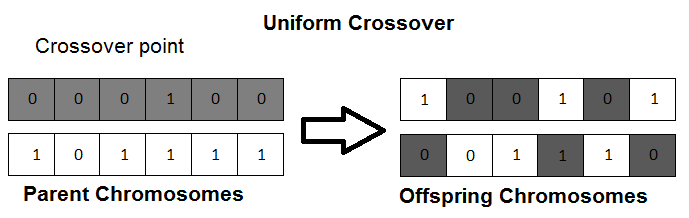
\includegraphics[width=7cm]{Crossover.png}
\caption{Uniformní křížení.}
\label{Crossover}
\end{wrapfigure}

Ke křížení použijeme uniformní metodu, kde každá bitová pozice potomka je vybrána z jednoho nebo druhého rodiče (s $50\%$ pravděpodobností) viz obr. \ref{Crossover}. 

Mutaci zajistíme jako náhodné překlopení bitu s pravděpodobností $10\%$ pro každý bit potomka.

Prvky generace seřadíme podle jejich fitness funkce připojíme nové prvky vzniklé křížením a odstraníme prvky s nejnižší hodnotou fitness funkce tak, aby populace měla opět 50 prvků.

Genetický algoritmus ukončíme po dosažení 150 generace prvků. Pro naši neuronovou síť použijeme parametry prvku s nejvyšší hodnotou fitness funkce z poslední generace.

\section{Výsledky}
Běh procesu optimalizace genetickým algoritmem trval 26 hodin a vybraný prvek obsahoval parametry dle tab. \ref{GABPNN_attributes}.

\begin{table}[h]
\centering
\begin{tabular}{ccc}
$\texttt{Parametr}$ & $\texttt{Bitová reprezentace}$ & $\texttt{Hodnota}$\\\hline
$\text{Počet skrytých neuronů}$ 	& $11111100$	& $252$		\\
$\text{Rychlost učení}$ 			& $000011001$	& $0,050781$		\\
$\text{Moment učení}$ 				& $111111000$	& $0,986328$		\\
\end{tabular}
\caption{Parametry neuronové sítě optimalizované genetickým algoritmem.\label{GABPNN_attributes}}
\end{table}
\vspace{\baselineskip}

\begin{wraptable}[8cm]{l}{7cm}
\begin{tabular}{cc}
$\texttt{Parametr}$ & $\texttt{Hodnota}$					\\\hline
$\text{Počet skrytých neuronů}$ 	& $72$		\\
$\text{Rychlost učení}$ 			& $0,2$		\\
$\text{Moment učení}$ 				& $0,9$		\\
\end{tabular}
\caption{Parametry neoptimalizované neuronové sítě.}
\label{BPNN_attributes}
\end{wraptable}

Trénování výsledné sítě probíhalo dokud hodnota MSE neklesnula pod hranici 0.00001. Pro natrénování sítě s parametry, které byli optimalizovány genetickým algoritmem, bylo potřeba průměrně 2230 trénovacích cyklů oproti 3725 cyklům pro obecnou síť \cite{thumb_rule} (viz tab. \ref{BPNN_attributes}).

\begin{table}[h]
\centering
\begin{tabular}{ccc}
$\texttt{Data}$ & $\texttt{Optimalizovaná}$ & $\texttt{Neoptimalizovaná}$\\\hline
$\text{Rozpoznání jednoho znaku}$ 	& $97,18\%$	& $96,94\%$		\\
$\text{Čas trénovacího cyklu}$ 		& $2,50ms$	& $1,38ms$		\\
$\text{Celkové rozpoznání značky}$ 	& $85,97\%$	& $84,62\%$		\\
\end{tabular}
\caption{Porovnání optimalizované a neoptimalizované sítě.}
\label{recognition_result}
\end{table}

\noindent
Z výsledků vyplývá že doba trénovacího cyklu je pro naši síť delší což je způsobeno použitím většího počtu neuronů ve skryté vrstvě sítě. Ovšem díky snížení počtu potřebných trénovacích cyklů došlo k celkovému zrychlení trénovacího procesu sítě. Tedy i snížení výpočetních nároků bez ztráty na rozpoznávací schopnosti sítě.

\bibliography{mybib}
\bibliographystyle{plain}
%\bibliography{References}
\end{document}